% Asset ID: AS1DifferentiationTIKZ-006
% Source: CCEA AS1-DIFF-LO004 and AS1-DIFF-LO005
% Related lesson section: Core Theory 18
% Purpose: Show derivative chain from y to dy/dx to d^2y/dx^2.

\documentclass[tikz,border=8pt]{standalone}
\usepackage{amsmath}
\usetikzlibrary{arrows.meta, positioning}

\begin{document}
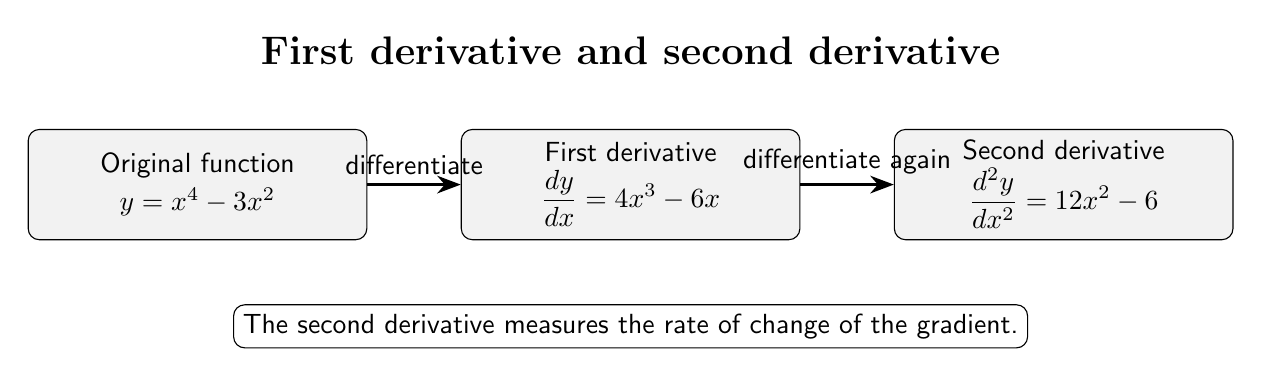
\begin{tikzpicture}[
    font=\sffamily,
    box/.style={draw, rounded corners, fill=gray!10, minimum width=4.3cm, minimum height=1.4cm, align=center},
    arrow/.style={thick, -{Stealth[length=3mm]}}
]

\node[font=\Large\bfseries] at (5.5,3.2) {First derivative and second derivative};

\node[box] (f) at (0,1.5) {Original function\\[2pt]$y=x^4-3x^2$};
\node[box] (fp) at (5.5,1.5) {First derivative\\[2pt]$\displaystyle \frac{dy}{dx}=4x^3-6x$};
\node[box] (fpp) at (11,1.5) {Second derivative\\[2pt]$\displaystyle \frac{d^2y}{dx^2}=12x^2-6$};

\draw[arrow] (f) -- node[above]{differentiate} (fp);
\draw[arrow] (fp) -- node[above]{differentiate again} (fpp);

\node[draw, rounded corners, fill=white, align=center] at (5.5,-0.3)
{The second derivative measures the rate of change of the gradient.};

\end{tikzpicture}
\end{document}
